\begin{frame}
  \begin{theorem}
    Si $f: D_{f} \subseteq \omega^{n} \times \Sigma^{\ast m} \rightarrow O$ es $\Sigma$-computable, entonces $f$ es
    $\Sigma$-Turing computable.
  \end{theorem}

  \begin{block}{Proof}
    \PN Supongamos $O = \SIGMA$. Por el Lema anterior, existe $\mathcal{P} \in \mathrm{Pro}^{\Sigma}$ el cual computa
    $f$ y tiene las propiedades (1) y (2). Sea $k = \max \{n, m, N(\mathcal{P})\}$ y sea $M_{sim}$ la máquina de Turing
    con unit que simula a $\mathcal{P}$ respecto de $k$. Como puede observarse, la máquina $M_{sim}$, no necesariamente
    computará a $f$. Sea $M_{1}$ la siguiente máquina:
  \end{block}

  \begin{figure}[h]
    \centering
    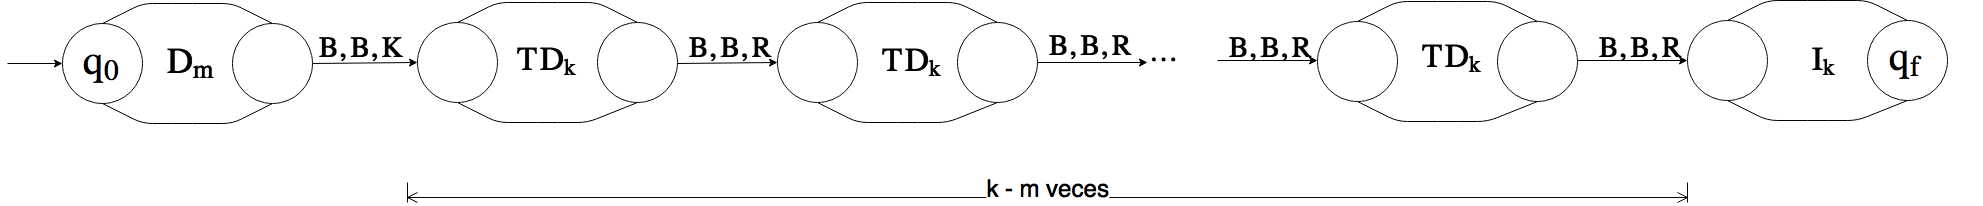
\includegraphics[scale=0.19]{graphics/figure_9.png}
  \end{figure}
\end{frame}
